\documentclass[conference]{IEEEtran}
\IEEEoverridecommandlockouts

\usepackage[T1]{fontenc}
\usepackage[utf8]{inputenc}
\usepackage[french]{babel}
\usepackage{cite}
\usepackage{amsmath,amssymb,amsfonts}
\usepackage{graphicx}
\usepackage{booktabs}
\usepackage[hidelinks]{hyperref}

\newcommand{\toolname}{\textsc{PerforceLog}}
\newcommand{\beepbeep}{\textsc{BeepBeep}}

\begin{document}

\title{Detecting Collaboration Antipatterns in Perforce Server Logs\\
with Stream Metrics and Complex Event Processing}

\author{%
\IEEEauthorblockN{Hanifah ALPHA-BODA}
\IEEEauthorblockA{\textit{Laboratoire d'informatique formelle}\\
\textit{Universit\'e du Qu\'ebec \`a Chicoutimi}\\
Chicoutimi, Canada\\
haboda@etu.uqac.ca}
\and
\IEEEauthorblockN{Yannick FRANCILETTE}
\IEEEauthorblockA{\textit{Laboratoire d'informatique formelle}\\
\textit{Universit\'e du Qu\'ebec \`a Chicoutimi}\\
Chicoutimi, Canada\\
yfrancil@uqac.ca}
\and
\IEEEauthorblockN{Sylvain HALL\'E}
\IEEEauthorblockA{\textit{Laboratoire d'informatique formelle}\\
\textit{Universit\'e du Qu\'ebec \`a Chicoutimi}\\
Chicoutimi, Canada\\
shalle@uqac.ca}
}

\maketitle

\begin{abstract}
Les serveurs de gestion de versions enregistrent chaque action d'une
équipe, mais ces journaux sont rarement exploités pour analyser la
collaboration. Dans l'industrie du jeu vidéo, des équipes nombreuses
partagent des dépôts volumineux de \textbf{fichiers binaires} non
fusionnables~: les signaux utiles proviennent des séquences d'opérations
(modification, synchronisation, soumission, annulation) et de leurs
durées, non de comparaisons de contenu textuel.

Nous présentons \toolname{}, une \textbf{contribution logicielle} qui
détecte des \emph{antipatterns de collaboration}---comportements
d'équipe récurrents et indésirables---à partir des journaux du serveur
Perforce. Cinq motifs du catalogue ReliSA (sur 168) sont
opérationnalisés. L'outil assemble des blocs d'événements puis enchaîne
deux traitements complémentaires~: métriques agrégées inspirées de
Prometheus~\cite{brazil2018prometheus,prometheus_metric_types}, puis
traitement d'événements complexes sensible à l'ordre des
actions~\cite{halle2018beepbeep,luckham2002power}.

Sur un journal de 1,7~Go, il extrait 16\,262 événements uniques en
${\sim}$14~s, signale 217 séquences \emph{modification-puis-annulation}
et 250 fichiers abandonnés~; une jauge indépendante confirme ce
décompte (250\,=\,250). Ces résultats montrent la faisabilité d'une
analyse automatique à grande échelle et la cohérence interne du pipeline
proposé.
\end{abstract}

\begin{IEEEkeywords}
traitement d'événements complexes, fouille de dépôts, antipatterns de
collaboration, Perforce, observabilité
\end{IEEEkeywords}

\section{Introduction}

\textbf{Contexte.}
Le développement de jeux vidéo repose sur de grandes équipes et des
outils de gestion de versions partagés. Les retards de production ont un
coût financier majeur pour les studios~; une collaboration dysfonctionnelle
contribue souvent à ces dérapages, même si elle reste difficile à
objectiver.

\textbf{Problématique.}
La recherche en génie logiciel s'intéresse de plus en plus aux
\emph{antipatterns de collaboration}~\cite{brown1998antipatterns,tamburri2019community,relisa_catalogue}~:
comportements d'équipe récurrents et contre-productifs. Les détecter tôt
permettrait une rétroaction avant qu'ils n'affectent la livraison.

\textbf{Problème.}
Les journaux serveur (\texttt{p4d} chez Perforce) enregistrent chaque
\texttt{edit}, \texttt{submit}, \texttt{sync} et \texttt{revert}, mais
atteignent facilement plusieurs gigaoctets de texte semi-structuré,
illisibles manuellement. Contrairement à Git, centré sur le graphe de
commits, Perforce journalise les opérations \emph{au niveau fichier}
(checkout, soumission, annulation), ce qui rend observable un fichier
«~ouvert mais jamais soumis~»---signal inaccessible aux approches
orientées commits~\cite{hindle2008mining}.

\textbf{Question de recherche.}
Comment analyser automatiquement ces journaux volumineux pour détecter
des mauvaises pratiques de collaboration, sans charger tout le fichier en
mémoire et en tenant compte de l'ordre des événements sur chaque
fichier~?

\textbf{Contributions.}
Il s'agit d'une contribution \textbf{appliquée} (outil reproductible),
non théorique~: (1)~parseur en flux par blocs d'événement
(\texttt{user-*} + \texttt{completed} + métriques, liés par
\texttt{pid})~; (2)~métriques de style Prometheus hors
ligne~\cite{openmetrics}~; (3)~automates pour motifs temporels.
\toolname{} opérationnalise \textbf{cinq} fiches ReliSA
(tableau~\ref{tab:relisa}).

\begin{table}[!t]
  \caption{Cinq antipatterns opérationnalisés (5/168 ReliSA).}
  \label{tab:relisa}
  \centering
  \small
  \begin{tabular}{ll}
    \toprule
    \textbf{Détection} & \textbf{Fiche ReliSA} \\
    \midrule
    Rush de submits & Collective\_Procrastination \\
    Faible activité (Warm Bodies) & Warm\_Bodies \\
    Ratio edit/submit (Lone Wolf) & Lone-Wolf \\
    Checkout sans submit (apathie) & Bystander\_Apathy \\
    Edit puis revert & Cascading\_Branches \\
    \bottomrule
  \end{tabular}
\end{table}

\section{\'Etat de l'art}
\label{sec:etat}

\textbf{Critères de sélection.}
Nous avons recensé les travaux sur (i)~la fouille de dépôts,
(ii)~les antipatterns et \emph{community smells}, (iii)~l'observabilité
par métriques, (iv)~le traitement d'événements complexes. La fenêtre
privilégiée est 2018--2026 (évolution rapide des chaînes
d'observabilité), avec références fondatrices plus anciennes si
nécessaire~\cite{luckham2002power,brown1998antipatterns}.

\textbf{Présentation.}
La fouille sur Git~\cite{hindle2008mining} analyse des commits en lot.
Les \emph{community smells}~\cite{tamburri2019community} ciblent des
signaux organisationnels souvent absents des journaux VCS. Prometheus
définit compteurs, jauges, histogrammes et
résumés~\cite{brazil2018prometheus,prometheus_metric_types}~;
OpenMetrics standardise leur
exposition~\cite{openmetrics}. \beepbeep{}~\cite{halle2018beepbeep}
unifie métriques et requêtes à état sur un flux Java.

\textbf{Comparaison.}
Le tableau~\ref{tab:comparaison} situe notre approche. Nous ciblons
explicitement les antipatterns de collaboration opérationnalisables sur
\texttt{p4d}, avec traitement en flux et mémoire d'ordre par fichier.

\begin{table}[!t]
  \caption{Comparaison synthétique (critères d'analyse).}
  \label{tab:comparaison}
  \centering
  \scriptsize
  \setlength{\tabcolsep}{2pt}
  \begin{tabular}{@{}lccccc@{}}
    \toprule
    \textbf{Approche} & \textbf{Flot} & \textbf{Ordre} & \textbf{\texttt{p4d}} & \textbf{Go} & \textbf{Collab.} \\
    \midrule
    Fouille Git~\cite{hindle2008mining} & \texttimes & \texttimes & \texttimes & \checkmark & partiel \\
    Community smells~\cite{tamburri2019community} & \texttimes & \texttimes & \texttimes & \checkmark & \checkmark \\
    Métriques Prometheus~\cite{prometheus_metric_types} & \checkmark & \texttimes & \texttimes & \checkmark & \texttimes \\
    \textbf{\toolname{} (notre)} & \checkmark & \checkmark & \checkmark & \checkmark & \checkmark \\
    \bottomrule
  \end{tabular}
\end{table}

\textbf{Discussion.}
Notre force est la combinaison \emph{échelle} (1,7~Go en ${\sim}$14~s),
\emph{granularité fichier} propre à Perforce et \emph{validation croisée}
entre métriques et automates. Compromis~: cinq proxies sur 168 fiches
ReliSA, seuils contextuels, pas encore de précision mesurée sur alertes
étiquetées.

\section{M\'ethodologie}
\label{sec:methodo}

\textbf{Catalogue et motifs.}
ReliSA~\cite{relisa_catalogue} recense 168 antipatterns~; nous en
implémentons cinq (tableau~\ref{tab:relisa}). Événement
$e{=}(t,u,f,a)$~; $E(u)$, $S(u)$ = \texttt{edit}/\texttt{submit}.
Motifs 1--3 (procrastination, Warm Bodies, Lone Wolf) en phase~1~;
4--5 (apathie, edit$\rightarrow$revert) en automates Moore (phase~2).
Chaque entrée de log référence des fichiers par chemin dépôt, tel que
documenté pour les commandes \texttt{user-*}~\cite{perforce_p4d}.

\textbf{Pipeline.}
\texttt{LecteurLog} assemble des blocs en streaming, déduplique, puis
\beepbeep{}~3.13 (fig.~\ref{fig:arch})~: dataset
\texttt{perforce\_events\_v3.json/.csv} (27 colonnes), quatre JSON de
métriques et \texttt{perforce\_events\_alertes.json}. Phase~1~:
Counter, Gauge ($+1$/\texttt{edit}, $-1$/\texttt{submit}/\texttt{revert}),
Histogram (16 buckets), Summary (p50, p95, p99). Phase~2~:
\texttt{edit}$\rightarrow$ouvert, \texttt{submit}$\rightarrow$fermé,
\texttt{revert} depuis ouvert $\rightarrow$alerte, ouvert en fin de flux
$\rightarrow$apathie~; rush si $\geq 3$ soumetteurs/heure. La jauge
terminale doit égaler les alertes d'apathie
(section~\ref{sec:resultats}).

\begin{figure}[!t]
  \centering
  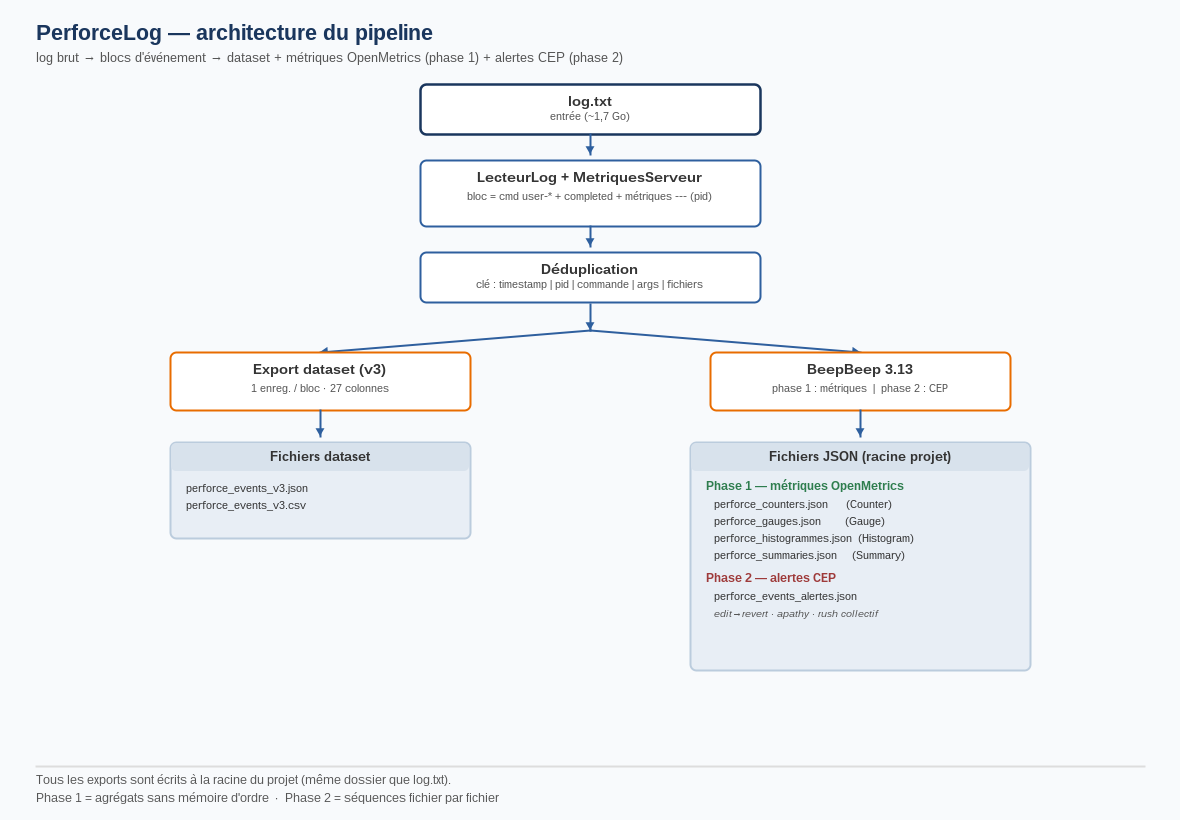
\includegraphics[width=\linewidth]{figures/fig00_architecture_pipeline.png}
  \caption{Pipeline \toolname{} (exports à la racine du projet).}
  \label{fig:arch}
\end{figure}

\section{R\'esultats}
\label{sec:resultats}

\textbf{Jeu de données.}
L'évaluation porte sur un journal de 1,7~Go collecté dans un
\textbf{cours} de développement de jeux multi-équipes (projet NAD/NAND,
moteur de jeu 5.6, 26--27~avril~2026)---contexte expérimental
contrôlé, distinct du déploiement industriel visé par l'outil. Traité en
${\sim}$14~s (tableau~\ref{tab:resume}).

\begin{table}[!t]
  \caption{Jeu de données et résultats principaux.}
  \label{tab:resume}
  \centering
  \scriptsize
  \setlength{\tabcolsep}{3pt}
  \begin{tabular}{@{}lr@{}}
    \toprule
    \multicolumn{2}{c}{\textit{Extraction}} \\
    \midrule
    Taille / blocs uniques / doublons & 1,7~Go / 16\,262 / 925 \\
    \texttt{edit} / \texttt{submit} / temps & 4\,069 / 1\,224 / ${\sim}$14~s \\
    \midrule
    \multicolumn{2}{c}{\textit{Activité (phase 1)}} \\
    \midrule
    Pic submits / utilisateurs (15~h) & 107 / 60 \\
    Pic jauge (fichiers / utilisateurs) & 500 / 79 \\
    ${\geq}$89\,\% commandes $<$0,25~s & moy.\ 7,36~s, méd.\ 0,094~s \\
    \midrule
    \multicolumn{2}{c}{\textit{Antipatterns (phase 2)}} \\
    \midrule
    Edit$\rightarrow$revert / apathie & 217 / 250 \\
    Validation jauge = apathie & 250 = 250 \\
    Lone Wolf max.\ (éd./soum.) & 364 / 2 ($\times$182) \\
    \bottomrule
  \end{tabular}
\end{table}

\textbf{Activité.}
Procrastination collective~: quasi nul la nuit, pic à \textbf{15~h}
(jour de remise), jusqu'à 60 utilisateurs actifs/heure
(fig.~\ref{fig:activite}, g.). La jauge de fichiers ouverts suit la même
dynamique (fig.~\ref{fig:activite}, d.), pic à 500 fichiers (79
utilisateurs).

\textbf{Durées.}
${\sim}$89\,\% des commandes $<$0,25~s~; une minorité de
\texttt{sync} sur fichiers binaires forme une longue traîne
(fig.~\ref{fig:metrics}, g.)~; \texttt{sync} p99\,=\,1\,102~s
(tab.~\ref{tab:quantiles}).

\begin{table}[!t]
  \caption{Quantiles Summary (secondes).}
  \label{tab:quantiles}
  \centering
  \scriptsize
  \begin{tabular}{@{}lrrr@{}}
    \toprule
    \textbf{Cmd.} & \textbf{p50} & \textbf{p95} & \textbf{p99} \\
    \midrule
    globale & 0,094 & 1,144 & 85,1 \\
    \texttt{edit} & 0,110 & 0,204 & 0,698 \\
    \texttt{submit} & 0,125 & 0,250 & 0,821 \\
    \texttt{sync} & 0,188 & 104,7 & 1\,102 \\
    \bottomrule
  \end{tabular}
\end{table}

\textbf{Antipatterns et validation.}
CEP~: 217 edit$\rightarrow$revert, 250 apathie, rush 60 utilisateurs/h
(27/04, 13~h) (fig.~\ref{fig:metrics}, d.). \textbf{Validation
croisée}~: jauge phase~1 et automate phase~2 concordent exactement
(250\,=\,250).

\begin{figure}[!t]
  \centering
  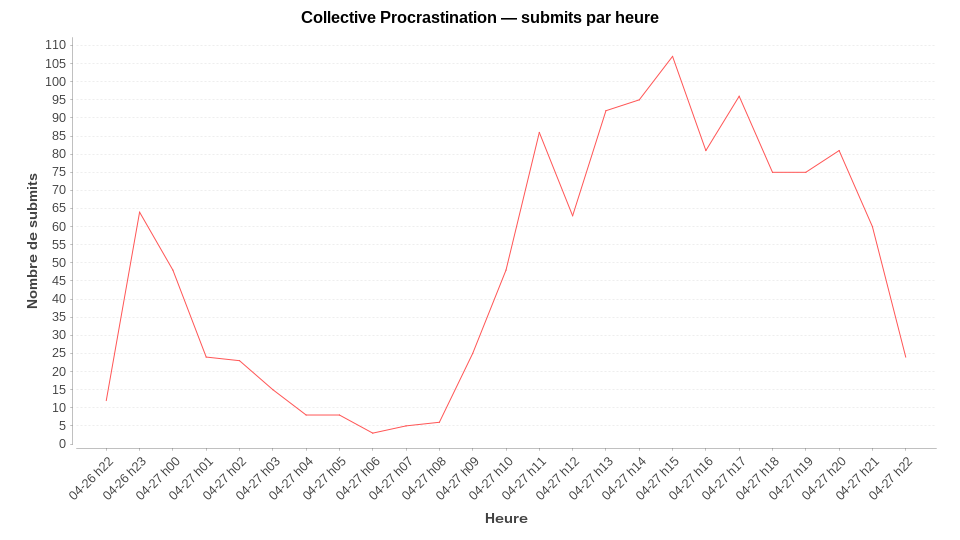
\includegraphics[width=0.48\linewidth]{figures/fig02_submits_par_heure.png}
  \hfill
  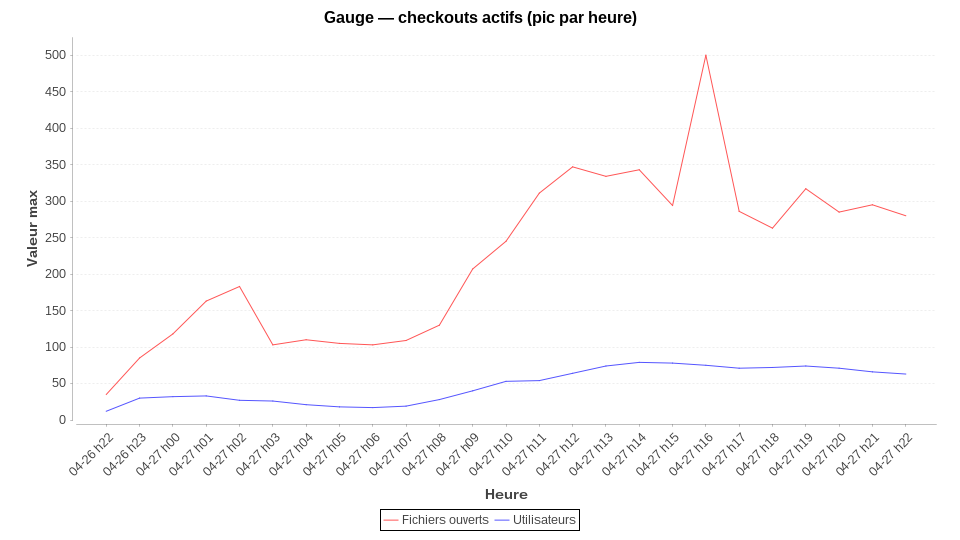
\includegraphics[width=0.48\linewidth]{figures/fig03_gauge_ouverts.png}
  \caption{Activité 24~h autour de l'échéance. \textbf{G.}~soumissions/heure
    (pic 107 à 15~h). \textbf{D.}~fichiers ouverts (pic 500).}
  \label{fig:activite}
\end{figure}

\begin{figure}[!t]
  \centering
  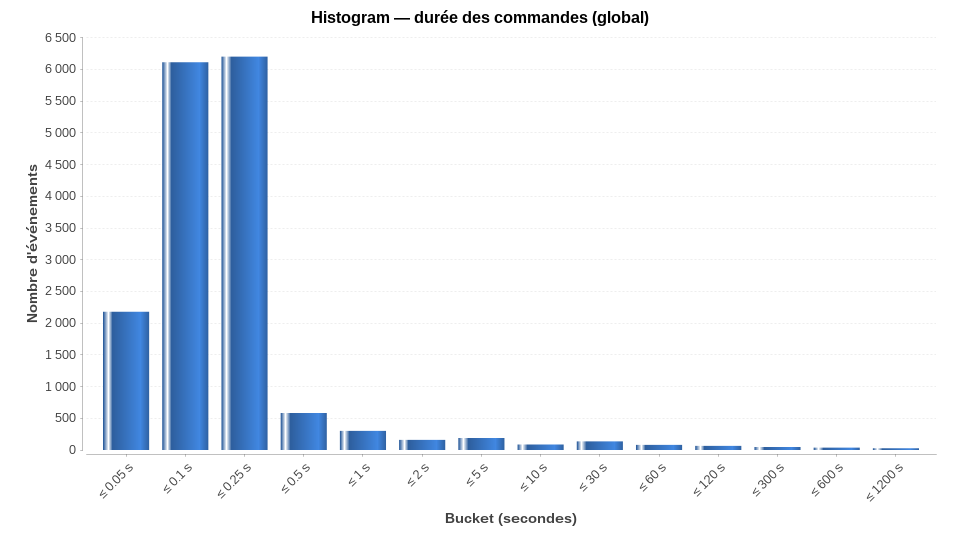
\includegraphics[width=0.48\linewidth]{figures/fig04_histogram_durees.png}
  \hfill
  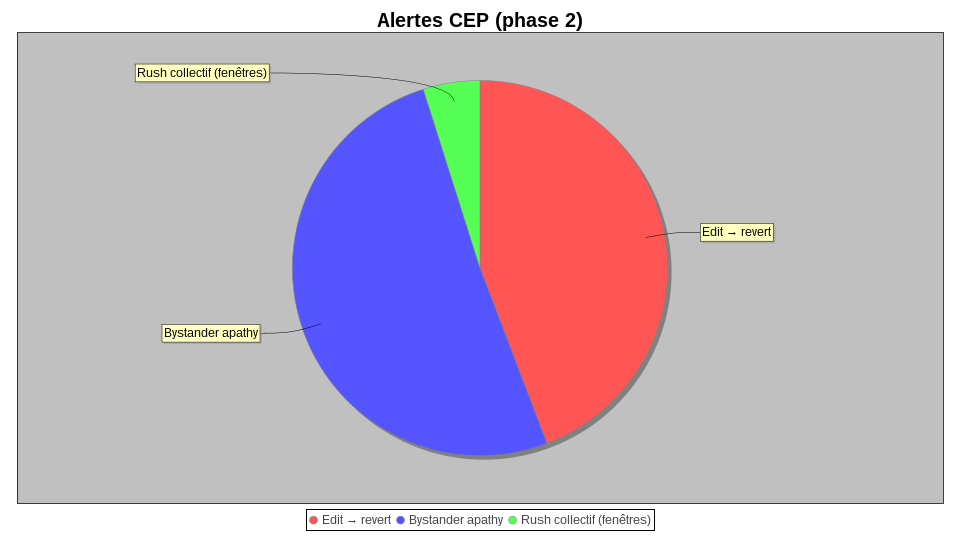
\includegraphics[width=0.48\linewidth]{figures/fig07_alertes_phase2.png}
  \caption{\textbf{G.}~durées (traîne de \texttt{sync} lentes).
    \textbf{D.}~alertes phase~2.}
  \label{fig:metrics}
\end{figure}

\section{Conclusion et limites}
\toolname{} est une contribution logicielle combinant métriques agrégées
et traitement d'événements complexes sur journaux Perforce. L'accord
jauge/apathie (250/250) illustre la cohérence interne des deux phases.

\textbf{Limites.} Cinq motifs sur 168 ReliSA~; seuils propres au jeu de
données~; log multi-projets~; validation d'alertes (précision) à
faire~; expérimentation sur cours, pas encore sur studio industriel.

\textbf{Perspectives.} Échantillon d'alertes étiqueté, tableaux de bord
par équipe, code open source, généralisation à d'autres journaux VCS au
niveau fichier.

\bibliographystyle{IEEEtran}
\bibliography{ieee_gem_references}

\end{document}
